\documentclass[11pt, a4paper]{article}

% ── Packages ──────────────────────────────────────────────────────────────────
\usepackage[top=1in, bottom=1in, left=1.1in, right=1.1in]{geometry}
\usepackage{booktabs}
\usepackage{tabularx}
\usepackage{array}
\usepackage{enumitem}
\usepackage{xcolor}
\usepackage{titlesec}
\usepackage{fancyhdr}
\usepackage{parskip}
% microtype letterspacing unsupported in XeTeX — omitted
\usepackage{graphicx}
\usepackage{amsmath}
\usepackage[hidelinks]{hyperref}
\usepackage{setspace}
\usepackage{caption}
\usepackage{colortbl}
\usepackage{mdframed}
\usepackage{tikz}
\usetikzlibrary{positioning}
\usepackage{multicol}
\usepackage{fontspec}

% ── Fonts ─────────────────────────────────────────────────────────────────────
\setmainfont{Georgia}
\setsansfont{Helvetica Neue}

% ── Colours ───────────────────────────────────────────────────────────────────
\definecolor{navyblue}{HTML}{00529B}
\definecolor{midblue}{HTML}{1A72B8}
\definecolor{lightblue}{HTML}{E8F1FA}
\definecolor{tableheader}{HTML}{1A72B8}
\definecolor{tablerow}{HTML}{EEF4FB}
\definecolor{darkgray}{HTML}{2C2C2C}
\definecolor{medgray}{HTML}{555555}
\definecolor{rulecol}{HTML}{2E86C1}
\definecolor{accentbar}{HTML}{00529B}

% ── Page style ────────────────────────────────────────────────────────────────
\pagestyle{fancy}
\fancyhf{}
\renewcommand{\headrulewidth}{0pt}
\fancyhead[L]{\small\color{medgray}\textsf{GenAI Capstone Project \textperiodcentered{} Solar Energy Forecasting}}
\fancyhead[R]{\small\color{medgray}\textsf{Milestones 1 \& 2}}
\fancyfoot[C]{\small\color{medgray}\textsf{\thepage}}

% ── Section styling ───────────────────────────────────────────────────────────
\titleformat{\section}
  {\large\bfseries\sffamily\color{navyblue}}
  {\thesection.}{0.6em}{}
  [\vspace{2pt}{\color{rulecol}\titlerule[0.8pt]}]

\titleformat{\subsection}
  {\normalsize\bfseries\sffamily\color{midblue}}
  {\thesubsection}{0.6em}{}

\titlespacing{\section}{0pt}{18pt}{8pt}
\titlespacing{\subsection}{0pt}{12pt}{4pt}

% ── Table helpers ─────────────────────────────────────────────────────────────
\newcommand{\thead}[1]{\cellcolor{tableheader}\color{white}\textsf{\textbf{#1}}}
\newcommand{\trow}{\rowcolor{tablerow}}
\newcolumntype{L}[1]{>{\raggedright\arraybackslash}p{#1}}
\newcolumntype{C}[1]{>{\centering\arraybackslash}p{#1}}

% ── Misc ──────────────────────────────────────────────────────────────────────
\setlist[itemize]{noitemsep, topsep=4pt, leftmargin=1.4em}
\setlist[enumerate]{noitemsep, topsep=4pt, leftmargin=1.6em}
\captionsetup{font=small, labelfont=bf, skip=4pt}
\color{darkgray}

% ──────────────────────────────────────────────────────────────────────────────
\begin{document}

% ── Title page ────────────────────────────────────────────────────────────────
\begin{titlepage}
\thispagestyle{empty}

% Top accent bar
\begin{tikzpicture}[remember picture, overlay]
  \fill[navyblue] (current page.north west) rectangle
    ([yshift=-3.2cm]current page.north east);
\end{tikzpicture}

\vspace*{1.2cm}

\begin{center}
  {\small\sffamily\color{white}\addfontfeatures{LetterSpace=12}MILESTONE 1 \& 2 \textperiodcentered{} PROJECT REPORT\addfontfeatures{LetterSpace=0}}\\[0.6cm]
  {\Huge\bfseries\sffamily\color{white} AI-Based Solar Energy\\[0.2cm] Forecasting System}\\[0.5cm]
  {\large\sffamily\color{white!80!navyblue}
    Machine Learning Pipeline for 15-Minute Ahead\\Solar Power Generation Forecasting}
\end{center}

\vspace{2.6cm}

\begin{center}
\begin{tabular}{@{} L{4cm} L{8cm} @{}}
\toprule
\textbf{Course}       & GenAI Capstone Project \\[3pt]
\textbf{Dataset}      & Kaggle Solar Power Generation Data (Plant 1 \& 2) \\[3pt]
\textbf{Repository}   & \href{https://github.com/Aviral02git/Solar-power-prediction}
                         {github.com/Aviral02git/Solar-power-prediction} \\[3pt]
\textbf{Deployed App} & \href{https://solarpowerpredictionmodel.streamlit.app/}
                         {solarpowerpredictionmodel.streamlit.app} \\[3pt]
\textbf{Date}         & April 2026 \\
\bottomrule
\end{tabular}
\end{center}

\vfill

\begin{center}
\begin{tabular}{@{} L{3.5cm} L{3.5cm} L{6cm} @{}}
\thead{Member} & \thead{Role} & \thead{Contributions} \\
\trow
Ved & Tech Lead &
  Model development, feature engineering, Streamlit deployment, system integration \\
Aviral Mishra & Data \& Quality Lead &
  Dataset preparation, data quality checks, preprocessing pipeline \\
\trow
Naitik Pandey & Report \& Evaluation Lead &
  Model evaluation, metric analysis, project documentation \\
Samarth Khera & Analysis Lead &
  Trend analysis, visualisation, insights from results \\
\end{tabular}
\end{center}

\vspace{0.8cm}
\end{titlepage}

% ── Table of Contents ─────────────────────────────────────────────────────────
\tableofcontents
\thispagestyle{empty}
\newpage
\setcounter{page}{1}

% ──────────────────────────────────────────────────────────────────────────────
\section{Introduction \& Problem Statement}

Solar energy generation is among the most cost-effective and scalable forms of renewable
power, yet its output is governed by meteorological conditions that change continuously.
Cloud cover, irradiance fluctuations, temperature gradients, and diurnal cycles mean that
plant-level DC power can vary by orders of magnitude within minutes. Grid operators cannot
absorb this variability passively — they require short-horizon forecasts to dispatch backup
generation, balance storage charge cycles, and preserve frequency stability.

This project builds a complete machine learning pipeline that ingests raw inverter-level
generation records and weather sensor readings from a real solar plant and produces a
15-minute ahead DC power forecast. The system is deployed as an interactive web application
through which a grid operator can upload daily plant data, inspect model performance, and
obtain structured optimisation recommendations from an autonomous agentic assistant.

\medskip
\noindent\textbf{Core problems addressed:}
\begin{itemize}
  \item Strong time-dependency in power output — successive 15-minute intervals are
        highly correlated, requiring lag-based features to capture temporal structure.
  \item Nonlinear relationships between irradiance, ambient temperature, module temperature,
        and plant-level generation that linear models cannot capture reliably.
  \item High variance during sunrise and sunset transition periods, where small changes
        in solar angle produce large swings in output.
  \item Noise in inverter-level measurements that must be aggregated before modelling.
  \item Grid operators need actionable, short-term guidance — not just a number — to
        allocate storage and schedule demand response.
\end{itemize}

% ──────────────────────────────────────────────────────────────────────────────
\section{System Evolution: Milestone 1 \texorpdfstring{$\rightarrow$}{->} Milestone 2}

The project was structured across two milestones. Milestone 1 delivered a classical ML
forecasting pipeline; Milestone 2 extended that pipeline with an agentic AI layer capable
of reasoning over forecast outputs and producing structured grid management recommendations.

\begin{table}[h]
\centering
\caption{Component-level comparison across milestones}
\begin{tabularx}{\textwidth}{@{} L{3.2cm} X X @{}}
\toprule
\thead{Component} & \thead{Milestone 1} & \thead{Milestone 2} \\
\midrule
\trow Core task     & 15-min solar power forecasting          & Agentic grid optimisation assistant \\
      Model         & RandomForestRegressor                   & RandomForest + LangGraph + LLM \\
\trow Retrieval     & None — static trained model             & FAISS vector search + MiniLM embeddings \\
      Pipeline      & Batch inference, single step            & Multi-node agentic workflow \\
\trow Output        & Numerical forecast + evaluation metrics & Structured optimisation recommendations \\
      Reasoning     & None (statistical inference)            & Multi-step LLM reasoning via Groq \\
\trow UI            & Streamlit — Tab 1 only                  & Streamlit — Tab 1 (forecast) + Tab 2 (agent) \\
\bottomrule
\end{tabularx}
\end{table}

% ──────────────────────────────────────────────────────────────────────────────
\section{Dataset}

The dataset was sourced from Kaggle's Solar Power Generation Data collection, which
contains real operational records from two solar plants in India, sampled at 15-minute
intervals over a 34-day period in May–June 2020.

\begin{table}[h]
\centering
\caption{Dataset files and key fields}
\begin{tabularx}{\textwidth}{@{} L{5.2cm} L{4.5cm} X @{}}
\toprule
\thead{File} & \thead{Key Fields} & \thead{Description} \\
\midrule
\trow \texttt{Plant\_1\_Generation\_Data.csv}
  & DATE\_TIME, DC\_POWER, PLANT\_ID, SOURCE\_KEY
  & Inverter-level DC power at 15-min intervals \\
\texttt{Plant\_1\_Weather\_Sensor\_Data.csv}
  & DATE\_TIME, AMBIENT\_TEMPERATURE, MODULE\_TEMPERATURE, IRRADIATION
  & Environmental sensor readings at plant level \\
\trow \texttt{Plant\_2\_Generation\_Data.csv}
  & Same schema as Plant 1
  & Second plant used for cross-plant validation \\
\texttt{Plant\_2\_Weather\_Sensor\_Data.csv}
  & Same schema as Plant 1
  & Weather data for Plant 2 \\
\bottomrule
\end{tabularx}
\end{table}

Plant 1 contains 68,778 inverter-level records across 22 inverters, which aggregate to
3,157 plant-level 15-minute timestamps after groupby summation. The weather sensor provides
one row per 15-minute interval at the plant level.

% ──────────────────────────────────────────────────────────────────────────────
\section{Methodology}

\subsection{Data Aggregation and Integration}

Inverter-level \texttt{DC\_POWER} readings are summed by timestamp to produce plant-level
output — a necessary step because the model must forecast total plant generation, not
per-inverter output. The aggregated generation table is then merged with the weather sensor
table on \texttt{DATE\_TIME}, and the result is sorted chronologically and stripped of any
rows containing nulls.

\subsection{Feature Engineering}

Nine features were constructed from the merged dataset. Three capture time periodicity
(\texttt{hour}, \texttt{day\_of\_year}, \texttt{month}); three capture temporal
autocorrelation in power output (\texttt{lag\_1}, \texttt{lag\_4}, \texttt{rolling\_mean\_4});
and three are direct environmental readings (\texttt{AMBIENT\_TEMPERATURE},
\texttt{MODULE\_TEMPERATURE}, \texttt{IRRADIATION}).

\begin{table}[h]
\centering
\caption{Feature engineering summary}
\begin{tabularx}{\textwidth}{@{} L{3.5cm} L{4.5cm} X @{}}
\toprule
\thead{Feature Type} & \thead{Features} & \thead{Rationale} \\
\midrule
\trow Time-based
  & \texttt{hour}, \texttt{day\_of\_year}, \texttt{month}
  & Captures diurnal and seasonal periodicity \\
Lag features
  & \texttt{dc\_power\_lag1} $(t{-}1)$, \texttt{dc\_power\_lag4} $(t{-}4)$
  & Recent history is the strongest predictor of near-future output \\
\trow Rolling statistic
  & \texttt{rolling\_mean\_4} (4-interval window)
  & Smooths short-term noise; tracks trend momentum \\
Weather features
  & \texttt{AMBIENT\_TEMPERATURE}, \texttt{MODULE\_TEMPERATURE}, \texttt{IRRADIATION}
  & Physical drivers of photovoltaic conversion efficiency \\
\trow Target variable
  & \texttt{DC\_POWER} shifted $-1$ interval
  & Defines the 15-minute ahead prediction objective \\
\bottomrule
\end{tabularx}
\end{table}

The target is formed by shifting \texttt{DC\_POWER} forward by one row, so each sample
represents the current state of the plant and the label is the plant's output in the next
15-minute interval.

\subsection{Model Training}

A \texttt{RandomForestRegressor} was selected as the primary model. Random forests handle
nonlinear feature interactions natively through recursive partitioning, require minimal
preprocessing, and are robust to the noisy inverter-level measurements present in the raw
data. The trained ensemble was persisted to \texttt{solar\_forecast\_model.pkl} via
\texttt{joblib} for inference in the Streamlit application.

\medskip
\noindent\textbf{Hyperparameters:}
\begin{itemize}
  \item \texttt{n\_estimators = 200}
  \item \texttt{max\_depth = 12}
  \item \texttt{random\_state = 42}
  \item \texttt{n\_jobs = -1} (parallelised across all cores)
\end{itemize}

Training was performed on the first 80\% of chronologically ordered records
(2,521 samples), with the remaining 20\% (631 samples) held out for evaluation.
A time-ordered split — rather than random shuffling — was used to prevent data leakage
across the temporal boundary.

% ──────────────────────────────────────────────────────────────────────────────
\section{System Architecture}

\subsection{Milestone 1 — Batch Inference Pipeline}

The Milestone 1 system follows a five-layer architecture in which each layer has a
single, well-defined responsibility.

\begin{table}[h]
\centering
\caption{Architectural layers}
\begin{tabularx}{\textwidth}{@{} L{0.5cm} L{4.2cm} X @{}}
\toprule
\thead{\#} & \thead{Layer} & \thead{Responsibility} \\
\midrule
\trow 1 & Data Layer
  & Ingestion of raw Plant Generation and Weather Sensor CSVs via Streamlit file uploader \\
2 & Feature Engineering Layer
  & Aggregation, timestamp alignment, lag features, rolling statistics, time-based features \\
\trow 3 & Machine Learning Layer
  & \texttt{RandomForestRegressor} inference using \texttt{solar\_forecast\_model.pkl} \\
4 & Evaluation Layer
  & MAE, RMSE, and $R^2$ computed against the held-out target column \\
\trow 5 & Application Layer
  & Streamlit UI rendering forecast chart, trend analysis, and downloadable predictions CSV \\
\bottomrule
\end{tabularx}
\end{table}

\subsection{Milestone 2 — Agentic Workflow Layer}

Milestone 2 introduces a \textbf{LangGraph} agentic layer that operates downstream of the
forecasting pipeline. After the Milestone 1 pipeline produces predictions, the agent
receives those predictions as input and executes a three-node directed workflow.

\medskip
\begin{center}
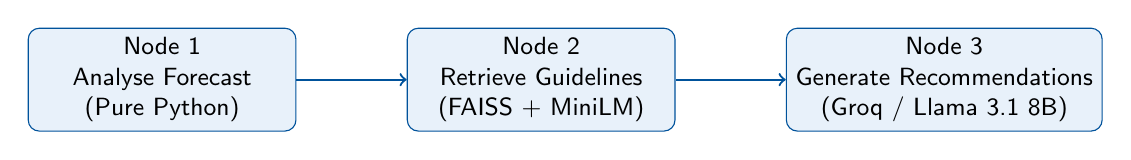
\begin{tikzpicture}[
  box/.style={
    draw=navyblue, fill=lightblue, rounded corners=4pt,
    minimum width=3.4cm, minimum height=1.1cm, align=center,
    font=\small\sffamily
  },
  arr/.style={->, thick, color=navyblue}
]
\node[box] (n1) {Node 1\\Analyse Forecast\\(Pure Python)};
\node[box, right=1.4cm of n1] (n2) {Node 2\\Retrieve Guidelines\\(FAISS + MiniLM)};
\node[box, right=1.4cm of n2] (n3) {Node 3\\Generate Recommendations\\(Groq / Llama 3.1~8B)};
\draw[arr] (n1) -- (n2);
\draw[arr] (n2) -- (n3);
\end{tikzpicture}
\end{center}
\medskip

\noindent\textbf{Node 1 — Analyse Forecast} (pure Python, no external calls):
Receives the full prediction array and irradiation series. Computes mean, max, min, standard
deviation, and variability percentage. Classifies grid risk as Low ($< 20\%$ variability),
Medium ($20$–$40\%$), or High ($> 40\%$). Identifies risk periods where output drops more than
30\% below the mean, and peak hours in the top decile of predicted output.

\medskip
\noindent\textbf{Node 2 — Retrieve Guidelines} (FAISS + sentence-transformers):
Constructs a semantic query from the Node 1 analysis output and performs a top-4 similarity
search over an in-memory FAISS index built from 18 grid management guideline chunks.
Embeddings are generated locally using \texttt{sentence-transformers/all-MiniLM-L6-v2},
with no external embedding API dependency.

\medskip
\noindent\textbf{Node 3 — Generate Recommendations} (Groq API, Llama 3.1~8B):
Sends the structured analysis and the four retrieved guideline passages to Llama 3.1~8B via
the Groq inference API. The model is prompted to return structured output — a forecast
summary, risk assessment, immediate actions, optimisation strategies, and referenced
guideline topics — without markdown formatting. JSON fence stripping is applied to the
response before parsing.

% ──────────────────────────────────────────────────────────────────────────────
\section{Technology Stack}

\begin{table}[h]
\centering
\caption{Full technology stack across both milestones}
\begin{tabularx}{\textwidth}{@{} L{3.2cm} X X @{}}
\toprule
\thead{Category} & \thead{Milestone 1} & \thead{Milestone 2 (additional)} \\
\midrule
\trow Language       & Python 3.11                          & Python 3.11 \\
      ML / Modelling & scikit-learn (RandomForestRegressor) & LangGraph, LangChain \\
\trow Vector search  & —                                    & FAISS + sentence-transformers (all-MiniLM-L6-v2) \\
      LLM inference  & —                                    & Groq API (Llama 3.1~8B) \\
\trow Data processing & Pandas 3.0, NumPy 2.4               & Pandas 3.0, NumPy 2.4 \\
      Visualisation  & Matplotlib 3.10                      & Matplotlib 3.10 \\
\trow Web UI         & Streamlit 1.54 — single tab          & Streamlit 1.54 — two tabs \\
      Model storage  & Joblib (.pkl)                        & Joblib (.pkl) \\
\trow Secrets        & \texttt{python-dotenv}               & \texttt{python-dotenv} + Streamlit secrets \\
      Dev environment & Google Colab                        & Google Colab / local venv \\
\bottomrule
\end{tabularx}
\end{table}

% ──────────────────────────────────────────────────────────────────────────────
\section{Evaluation \& Results}

Model performance was evaluated on the chronological 20\% hold-out split using three
standard regression metrics. Additionally, a daytime-only evaluation was performed by
filtering to hours with non-zero irradiation, isolating the model's performance under
the conditions where forecasting accuracy is most operationally relevant.

\begin{table}[h]
\centering
\caption{Model evaluation results}
\begin{tabularx}{\textwidth}{@{} L{3.5cm} C{2.2cm} C{2.5cm} C{1.8cm} X @{}}
\toprule
\thead{Evaluation Split} & \thead{MAE} & \thead{RMSE} & \thead{$R^2$} & \thead{Observation} \\
\midrule
\trow Daytime only & 4,646.83 & 7,397.92 & 0.9905
  & Near-perfect accuracy under stable irradiance conditions \\
Full dataset & 10,573.81 & 21,207.71 & 0.9323
  & Reduced accuracy driven by sunrise and sunset transitions \\
\bottomrule
\end{tabularx}
\end{table}

An $R^2$ of 0.9905 on daytime-only data confirms that the model captures the underlying
photovoltaic generation process with high fidelity when irradiance is stable. The drop to
0.9323 on the full dataset reflects the difficulty of transition periods — dawn and dusk
introduce steep, short-lived power ramps that are structurally harder to predict with
lag-based features trained primarily on steady-state conditions.

The most informative feature, by a wide margin, was \texttt{IRRADIATION} (mean decrease in
impurity $> 0.8$). Lag features and rolling mean contributed the next largest shares,
confirming that temporal autocorrelation in power output carries predictive signal
independent of the weather variables.

% ──────────────────────────────────────────────────────────────────────────────
\section{Streamlit Application}

The application is structured across two tabs, each handling a distinct stage of the
analysis workflow.

\begin{table}[h]
\centering
\caption{Application features by tab}
\begin{tabularx}{\textwidth}{@{} L{2.8cm} L{3.8cm} X @{}}
\toprule
\thead{Tab} & \thead{Feature} & \thead{Description} \\
\midrule
\trow Tab 1 — Forecast & CSV upload
  & Accepts Plant Generation and Weather Sensor CSVs; validates required columns \\
Tab 1 — Forecast & Auto preprocessing
  & Aggregation, merge, feature engineering, and model inference applied automatically \\
\trow Tab 1 — Forecast & 15-min forecast chart
  & Actual vs. predicted DC power over a user-selected window (50–1,000 points) \\
Tab 1 — Forecast & Performance metrics
  & MAE, RMSE, and $R^2$ displayed as metric cards \\
\trow Tab 1 — Forecast & Anomaly detection
  & Points where prediction error exceeds a configurable threshold are flagged and highlighted \\
Tab 1 — Forecast & Trend analysis
  & Hourly bar chart and irradiation scatter plot \\
\trow Tab 1 — Forecast & Download predictions
  & Exports timestamp, actual, predicted, error, and anomaly flag as CSV \\
Tab 2 — AI Agent & Run Analysis
  & Triggers the LangGraph pipeline; results persist in session state across reruns \\
\trow Tab 2 — AI Agent & Grid recommendations
  & Structured risk assessment, actions, and optimisation strategies from Llama 3.1~8B \\
Tab 2 — AI Agent & Follow-up chat
  & Conversational interface for querying the analysis using RAG context \\
\trow Tab 2 — AI Agent & PDF report
  & Exports a LaTeX-compiled PDF containing analysis statistics and recommendations \\
\bottomrule
\end{tabularx}
\end{table}

\medskip
\noindent\textbf{Run locally:}
\begin{mdframed}[backgroundcolor=black!6, linewidth=0pt, innerleftmargin=10pt,
                 innertopmargin=6pt, innerbottommargin=6pt]
\texttt{\small python3 -m streamlit run app.py}
\end{mdframed}

% ──────────────────────────────────────────────────────────────────────────────
\section{Design Decisions \& Tradeoffs}

Every architectural choice in this project involved a tradeoff between capability, complexity,
and deployment constraints. The decisions below reflect practical engineering priorities for
a capstone project that must be reproducible, demonstrable, and academically rigorous.

\begin{table}[h]
\centering
\caption{Key design decisions with rationale and tradeoffs}
\begin{tabularx}{\textwidth}{@{} L{3.8cm} X L{4.2cm} @{}}
\toprule
\thead{Decision} & \thead{Rationale} & \thead{Tradeoff} \\
\midrule
\trow RandomForest over LSTM
  & Handles nonlinear tabular data; straightforward to train, interpret, and deploy without GPU
  & No explicit temporal memory; LSTM or TCN would model long-range dependencies better \\
Batch inference over real-time
  & Lower infrastructure complexity; appropriate for academic demonstration on static CSVs
  & Cannot respond to streaming grid inputs; not suitable for production without an API layer \\
\trow Groq / Llama 3.1~8B for Milestone 2
  & Fast inference, free-tier availability, strong instruction-following on structured output tasks
  & External API dependency; potential latency under load; cost at production scale \\
FAISS for RAG retrieval
  & Local, in-memory vector search with no external database dependency; zero network calls
  & Static knowledge base — index must be rebuilt to incorporate new guidelines \\
\trow Streamlit for UI
  & Rapid prototyping; one-command deployment to Streamlit Cloud; Python-native
  & Batch-only interaction model; no WebSocket support for streaming inference \\
\bottomrule
\end{tabularx}
\end{table}

% ──────────────────────────────────────────────────────────────────────────────
\section{Limitations \& Future Work}

\begin{table}[h]
\centering
\caption{Current limitations and planned improvements}
\begin{tabularx}{\textwidth}{@{} L{2.5cm} X X @{}}
\toprule
\thead{Category} & \thead{Current Limitation} & \thead{Planned Improvement} \\
\midrule
\trow Forecasting & Batch-only; no real-time data ingestion & Real-time streaming via Kafka + REST API layer \\
Model & No hyperparameter tuning & Add GridSearchCV / Optuna HPO pipeline \\
\trow Model & No cross-validation pipeline & Implement time-series cross-validation (TimeSeriesCV) \\
Architecture & No model drift detection & Add monitoring dashboard for production drift \\
\trow Architecture & No REST API endpoint & Deploy model as FastAPI REST service \\
ML Approach & RandomForest lacks temporal memory
  & Implement LSTM or Temporal Convolutional Networks \\
\trow Data & No live weather forecast integration & Integrate weather API for real-time future inputs \\
LLM (M2) & API latency and cost at scale & Cache recommendations; explore local LLM hosting \\
\trow LLM (M2) & Potential hallucination in recommendations
  & Add citation validation and fact-checking layer \\
\bottomrule
\end{tabularx}
\end{table}

% ──────────────────────────────────────────────────────────────────────────────
\section{Repository Structure}

\begin{mdframed}[backgroundcolor=black!5, linewidth=0pt, innerleftmargin=10pt,
                 innertopmargin=8pt, innerbottommargin=8pt]
{\small\ttfamily
\noindent Genai capstone/\\
\hspace*{1em}app.py\hspace{5.5em}Unified Streamlit app (Tab 1: forecast, Tab 2: AI agent)\\
\hspace*{1em}agent.py\hspace{4.6em}LangGraph 3-node agentic workflow + chat function\\
\hspace*{1em}rag.py\hspace{5.6em}FAISS vector store and retrieval function\\
\hspace*{1em}knowledge\_base.py\hspace{0.5em}18 grid management guideline text chunks\\
\hspace*{1em}report.tex\hspace{4em}This document\\
\hspace*{1em}requirements.txt\hspace{2em}Pinned Python dependencies\\
\hspace*{1em}data/\\
\hspace*{2em}Plant\_1\_Generation\_Data.csv\\
\hspace*{2em}Plant\_1\_Weather\_Sensor\_Data.csv\\
\hspace*{2em}Plant\_2\_Generation\_Data.csv\\
\hspace*{2em}Plant\_2\_Weather\_Sensor\_Data.csv\\
\hspace*{1em}milestone\_1/\\
\hspace*{2em}app.py\hspace{3.8em}Original Milestone 1 Streamlit app\\
\hspace*{2em}solar\_model.ipynb\hspace{0.2em}Training notebook (RandomForest)\\
\hspace*{2em}ARCHITECTURE.md\\
}
\end{mdframed}

% ──────────────────────────────────────────────────────────────────────────────
\section{Conclusion}

Milestone 1 delivers a complete, deployable machine learning pipeline for short-term solar
power forecasting. A RandomForestRegressor trained on temporally engineered features from
real plant operational data achieves an $R^2$ of 0.9905 under stable daytime conditions and
0.9323 across the full dataset — performance sufficient for operational use in grid
scheduling applications.

Milestone 2 extends this system into an agentic platform. Rather than producing a number
and stopping, the system now analyses forecast variability, retrieves relevant grid
management guidelines from a curated knowledge base, and synthesises structured
recommendations through multi-step LLM reasoning. This positions the system as a decision
support tool for grid operators, not merely a forecasting service.

The architecture is modular at every layer: the ML pipeline, the vector store, the LLM
integration, and the UI are independently replaceable components. Substituting the
RandomForest with an LSTM, swapping FAISS for a hosted vector database, or replacing
Groq with a locally hosted model each require changes to a single module. This modularity
is the principal engineering contribution of the project — it demonstrates how a GenAI
system can be constructed from composable, well-bounded components rather than as a
monolithic pipeline.

\vspace{1.5cm}
\begin{center}
  
\begin{tikzpicture}
    \fill[navyblue] (0,0) rectangle (\textwidth, 0.8pt);
  \end{tikzpicture}\\[6pt]
  {\small\sffamily\color{medgray}
    GenAI Capstone Project \textperiodcentered{} Solar Power Prediction \textperiodcentered{}
    \href{https://github.com/Aviral02git/Solar-power-prediction}
         {github.com/Aviral02git/Solar-power-prediction}
  }
\end{center}

\end{document}
